% !TeX program = xelatex
% AKeyS 视频问答算法复现报告
% 文档结构参照 docs/template/复现报告/main.tex
\documentclass[12pt,UTF8]{ctexart}
\usepackage{amsmath}
\usepackage{booktabs}
\usepackage{graphicx}
\usepackage{geometry}
\usepackage{caption}
\usepackage[hidelinks]{hyperref}
\geometry{a4paper,margin=2.5cm}
\captionsetup{labelsep=quad}
\allowdisplaybreaks

\title{AKeyS 视频问答算法复现报告}
\author{}
\date{2026 年 11 月 12 日}

\begin{document}
\maketitle

\section{实验}

本节在 EgoSchema Subset 的 500 个五选一视频问答样本上复现 AKeyS
（Agentic Keyframe Search）的问题引导关键帧搜索机制，将原实现的 GPT-4o 后端替换为
DeepSeek，并与均匀采样 18 帧、24 帧两组基线进行比较。实验直接使用官方提供的 LaViLa
帧级字幕，不重新执行视频解码、字幕生成或视觉模型推理，因此无需 GPU。三组实验采用
相同问题、字幕、语言模型和生成参数，结果文件均保存在代码仓中。

\subsection{实验设置}

\subsubsection{数据集与任务}

EgoSchema 是面向长视频理解的第一视角视频问答数据集。本实验使用原仓库附带的
EgoSchema Subset 标注与字幕，共 500 个样本，每个样本包含一个问题、五个候选答案和
一个正确答案编号。每个视频对应 180 条按时间排列的 LaViLa 字幕，可理解为按 1 fps
组织的 180 帧文本描述。字幕中的 \texttt{\#C} 表示拍摄者行为，\texttt{\#O} 表示其他
人物行为。程序读取 \texttt{data/egoschema/subset\_anno.json} 与
\texttt{data/egoschema/lavila\_subset.json}，二者按视频 ID 一一对应。数据概况见
表~\ref{tab:dataset}。

\begin{table}[htbp]
  \centering\small
  \caption{数据集与输入形式}
  \label{tab:dataset}
  \begin{tabular}{ll}
    \toprule
    项目 & 设置 \\
    \midrule
    数据集 & EgoSchema Subset \\
    样本数 & 500 个五选一问答样本 \\
    文本输入 & 官方 LaViLa 字幕，每视频 180 条 \\
    视频与视觉推理 & 本实验不读取原始视频，不运行视觉模型 \\
    数据划分 & 三组实验使用完全相同的 500 个视频 ID \\
    \bottomrule
  \end{tabular}
\end{table}

\subsubsection{实验平台与软件环境}

复现程序为本地命令行应用，计算开销主要来自 DeepSeek 网络 API，不需要 CUDA 或训练用
GPU。提供的 DeepSeek 脚本面向 Windows Git Bash，使用 \texttt{.venv/Scripts/python}；
在其他操作系统上可将解释器路径改为虚拟环境中的 \texttt{python}。依赖由
\texttt{requirements.txt} 固定，其中 OpenAI Python SDK 版本为 1.63.2，并针对
Python 3.14 前后的 NumPy、Matplotlib、OpenCV、pandas 和 Pillow 分别选择兼容版本。
运行过程需要稳定网络和有效的 DeepSeek API 密钥。

\subsubsection{评价指标}

主要指标为准确率与平均使用帧数。设样本数为 $N$，第 $i$ 个样本的预测答案和标签分别为
$\hat y_i$、$y_i$，实际读取的不同字幕帧数为 $f_i$，则
\begin{equation}
  \mathrm{Accuracy}=\frac{1}{N}\sum_{i=1}^{N}\mathbf{1}(\hat y_i=y_i),\qquad
  \overline F=\frac{1}{N}\sum_{i=1}^{N}f_i .
  \label{eq:metrics}
\end{equation}
答案解析失败或样本执行异常均保留在分母中并计为答错，不采用随机答案补齐。辅助指标包括
成功 API 调用数、缓存命中数、输入/输出 token 数、缓存输入 token 数和估算费用。费用为
离线汇总值，不替代服务商账单。三组实验的解析失败率均为 0，因此按全部样本与仅按已回答
样本计算的准确率一致。

\subsubsection{对比原则}

三组实验均使用 \texttt{deepseek-flash}，temperature 为 0.2，最大输出为 1024 token，
DeepSeek 思考模式关闭。均匀 24 帧是主要基线，其固定帧预算接近 AKeyS 官方报告的平均帧数；
均匀 18 帧用于观察较低固定预算下的表现。比较属于同一文本输入、同一后端下的描述性对照，
不与原论文使用 GPT-4o 的结果作严格等价比较，也不据单次运行推断统计显著性。

\subsection{AKeyS 实验配置}

\subsubsection{方法实现}

AKeyS 将视频帧及其时间段组织为动态搜索树。程序先以间隔 10 从 180 条字幕中取得 18 条
初始字幕，再执行“作答与置信度判断—搜索扩展”的循环。每轮包含两条互补推理路径：
一条先生成视频时序摘要，再结合摘要、字幕与问题作答并给出 1 至 5 级置信度；另一条直接
基于字幕推理作答，再由自评模块给出 1 至 3 级置信度。主流程采用
\texttt{vote\_conf\_and}：仅当两条路径答案一致，且摘要路径置信度不低于 3、反思路径
置信度不低于 3 时提前输出。

若信息不足，规划器根据问题、当前字幕和候选时间段选择最值得细分的时间段。本实验采用
\texttt{a\_star} 策略，每轮最多执行 5 次节点选择（\texttt{beam\_size=5}），不感兴趣段
采用 \texttt{retain} 保留，所有已访问帧编号用于最终帧数统计。搜索最多 5 步。达到最大
步数仍未产生可信一致答案时，后处理采用 \texttt{vote} 比较两条路径的答案；仍不一致则
调用一次直接 JSON 作答作为兜底。该过程对应代码中的
\texttt{main.py}、\texttt{summarizer.py} 与 \texttt{video\_seg.py}。

\subsubsection{DeepSeek 后端适配与工程改动}

原仓库通过 OpenAI Python SDK 调用 GPT-4o。本次复现保留其接口形式，将 base URL 设为
\texttt{https://api.deepseek.com}，模型名设为 \texttt{deepseek-flash}，并传入关闭思考的
请求参数。为支持完整 500 样本运行和审计，代码增加或完善了以下功能：
（1）按运行 ID、样本 ID 和调用类型记录原始响应及 token 用量；
（2）对限流、连接错误和超时进行最多三次尝试，并将 API 错误写入日志；
（3）缓存读写加锁，使用临时文件原子替换缓存，支持并发样本处理；
（4）单样本异常时仍输出结构化结果，避免整批任务丢失；
（5）统一 UTF-8 文件读写，补充 Python 3.14 依赖条件；
（6）新增独立均匀采样程序与离线汇总程序。API 密钥仅从环境变量或用户指定文件读取，
不写入代码、结果或文档。

\begin{table}[htbp]
  \centering\small
  \caption{AKeyS 复现实验参数}
  \label{tab:akeys-config}
  \begin{tabular}{ll}
    \toprule
    设置 & 数值 \\
    \midrule
    模型与 API & \texttt{deepseek-flash}，DeepSeek OpenAI 兼容接口 \\
    temperature / max tokens & 0.2 / 1024 \\
    思考模式 & 关闭（\texttt{thinking: disabled}） \\
    初始采样 & 间隔 10，共 18 帧字幕 \\
    搜索策略 & A$^*$，\texttt{beam\_size=5}，\texttt{final\_step=5} \\
    主流程答案模式 & \texttt{vote\_conf\_and}，两路置信度阈值均为 3 \\
    后处理与兜底 & \texttt{vote}；仍无一致答案时直接作答 \\
    并行与随机种子 & \texttt{max\_workers=1}；随机种子 42 \\
    缓存 & \texttt{cache/deepseek\_flash.pkl}，与 GPT-4o 缓存分离 \\
    \bottomrule
  \end{tabular}
\end{table}

\subsection{均匀采样基线}

独立程序 \texttt{uniform\_baseline.py} 使用 \texttt{numpy.linspace} 从每段视频的 180 条
字幕中均匀抽取 18 条或 24 条，连同相同问题和选项一次性输入 DeepSeek，要求模型返回
\texttt{final\_answer} 字段。基线不生成时序摘要，不评估置信度，不执行时间段扩展、后处理
投票或自我反思。每个样本只发起一次 API 请求，帧数固定为 18 或 24。除采样和推理流程外，
模型、temperature、最大输出 token、数据顺序和评价方式均与 AKeyS 一致。

\subsection{方法对比结果}

表~\ref{tab:results} 汇总三组完整 500 样本实验。AKeyS 答对 350 题，准确率为 70.0\%，
比均匀 24 帧基线高 3.4 个百分点，比均匀 18 帧基线高 4.2 个百分点；平均使用 22.508 帧，
比 24 帧基线少 1.492 帧，降幅约 6.2\%。因此，本次复现同时观察到准确率提升和相对 24 帧
基线的帧数下降。均匀采样从 18 帧增加到 24 帧仅提高 0.8 个百分点，说明在该设置下单纯
增加固定帧预算的收益有限。

\begin{table}[htbp]
  \centering\small
  \caption{EgoSchema Subset 500 个样本上的对比结果}
  \label{tab:results}
  \begin{tabular}{lccccc}
    \toprule
    方法 & 答对数 & 准确率$\uparrow$ & 平均帧数$\downarrow$ & 解析失败率 & API 错误 \\
    \midrule
    均匀采样 18 帧 & 329 / 500 & 65.8\% & 18.000 & 0 & 0 \\
    均匀采样 24 帧 & 333 / 500 & 66.6\% & 24.000 & 0 & 0 \\
    \textbf{AKeyS-A$^*$} & \textbf{350 / 500} & \textbf{70.0\%} & \textbf{22.508} & \textbf{0} & \textbf{0} \\
    \bottomrule
  \end{tabular}
\end{table}

\begin{figure}[htbp]
  \centering
  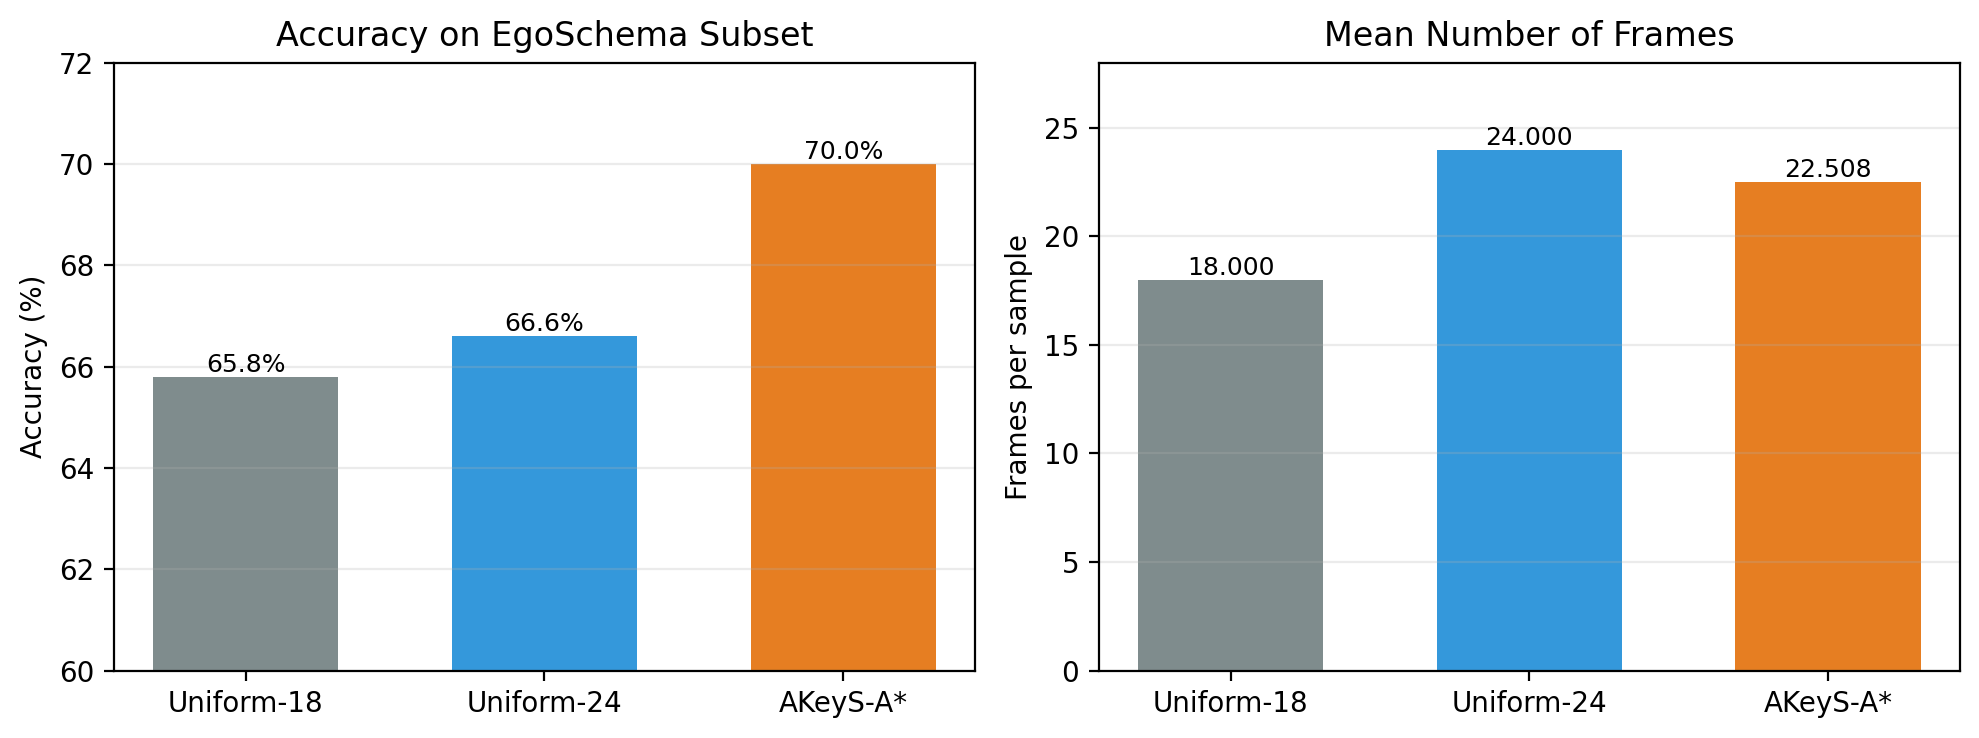
\includegraphics[width=\textwidth]{figures/fig_accuracy_frames.png}
  \caption{三种方法的准确率与平均使用帧数；数据由三组结果 JSON 直接生成}
  \label{fig:accuracy-frames}
\end{figure}

逐样本配对比较显示，相对均匀 24 帧基线，AKeyS 有 50 个样本由错转对、33 个样本由对转错，
两种方法同时答对 300 题、同时答错 117 题，净增 17 题。该结果说明提升并非所有样本的一致
改善，搜索策略仍会改变部分样本的答案；单次运行结果应结合这一波动理解。

\subsection{搜索过程与资源开销}

AKeyS 的帧数分布和答案产生阶段见图~\ref{fig:search-analysis}。250 个样本在第一步即满足
双路径一致及置信度条件，只使用 18 帧；440 个样本在主循环或后处理投票阶段完成，60 个样本
进入最终直接作答。全部样本使用帧数介于 18 和 41 之间，中位数为 19.5，第 90 百分位为 30。
答案产生阶段的细分统计见表~\ref{tab:stages}。兜底直接作答组的准确率为 50.0\%，低于第一步
完成组的 79.2\%，符合“较难或信息不明确样本需要更多搜索”的预期，但该分组准确率是事后
描述，不能单独证明搜索的因果收益。

\begin{figure}[htbp]
  \centering
  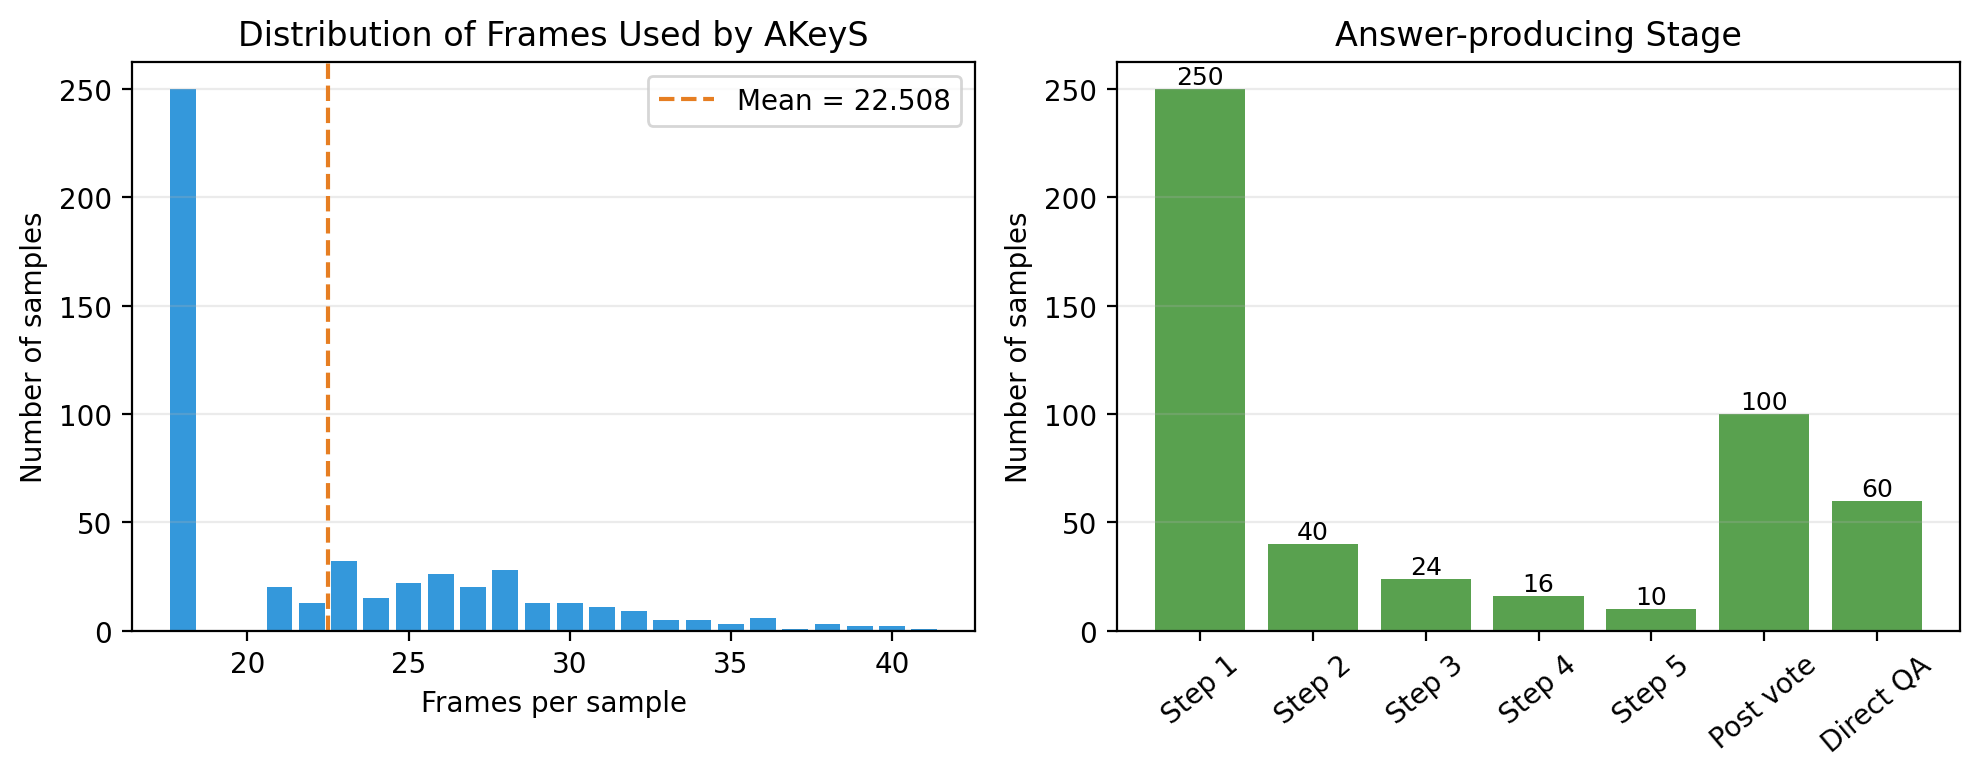
\includegraphics[width=\textwidth]{figures/fig_search_analysis.png}
  \caption{AKeyS 使用帧数分布与答案产生阶段统计}
  \label{fig:search-analysis}
\end{figure}

\begin{table}[htbp]
  \centering\small
  \caption{AKeyS 各答案产生阶段的样本数与表现}
  \label{tab:stages}
  \begin{tabular}{lcccc}
    \toprule
    阶段 & 样本数 & 答对数 & 阶段准确率 & 平均累计帧数 \\
    \midrule
    第 1 步一致作答 & 250 & 198 & 79.2\% & 18.000 \\
    第 2 步一致作答 & 40 & 29 & 72.5\% & 22.225 \\
    第 3 步一致作答 & 24 & 14 & 58.3\% & 25.583 \\
    第 4 步一致作答 & 16 & 11 & 68.8\% & 28.625 \\
    第 5 步一致作答 & 10 & 5 & 50.0\% & 29.100 \\
    后处理投票 & 100 & 63 & 63.0\% & 28.030 \\
    最终直接作答 & 60 & 30 & 50.0\% & 28.317 \\
    \bottomrule
  \end{tabular}
\end{table}

帧数较少并不等于 API 成本较低。AKeyS 在一个样本内会多次调用摘要、问答、规划、置信度
评估等模块；均匀基线每样本只调用一次。表~\ref{tab:cost} 按复现脚本中的单价估算费用：
非缓存输入 0.3 美元/百万 token、缓存输入 0.006 美元/百万 token、输出 1.2 美元/百万 token。
这些单价仅用于复现记录，实际费用应以运行时的服务商价格和账单为准。

\begin{table}[htbp]
  \centering\scriptsize
  \setlength{\tabcolsep}{4pt}
  \caption{API 调用、token 与估算费用}
  \label{tab:cost}
  \begin{tabular}{lrrrrr}
    \toprule
    方法 & 成功调用 & 缓存命中 & 总 token & 估算费用/美元 & 每答对题费用/美元 \\
    \midrule
    均匀 18 帧 & 500 & 0 & 309,383 & 0.095965 & 0.000292 \\
    均匀 24 帧 & 500 & 0 & 352,931 & 0.109029 & 0.000327 \\
    AKeyS-A$^*$ & 10,319 & 5,452 & 16,084,512 & 3.885545 & 0.011102 \\
    \bottomrule
  \end{tabular}
\end{table}

AKeyS 的 16,084,512 个总 token 中，输入为 14,857,814，输出为 1,226,698，其中缓存输入
6,951,826 token。其估算费用约为均匀 24 帧的 35.6 倍。因此，本次结果支持 AKeyS 在
“字幕帧数—准确率”维度上的有效性，但也表明实际部署必须同时考虑多轮语言模型调用的
延迟和费用，不能仅用平均帧数代表总计算成本。

\subsection{复现流程}

{\sloppy
完整代码、数据子集、结果和文档位于
\url{https://github.com/BolavenOfBrokenDream/AKeyS-re}。在仓库根目录创建虚拟环境并安装
\texttt{requirements.txt}，将 DeepSeek 密钥设置为环境变量 \texttt{OPENAI\_API\_KEY} 后，
先执行 \texttt{bash scripts/deepseek\_smoke.sh} 完成 5 样本检查，再执行
\texttt{bash scripts/deepseek\_full.sh} 依次运行均匀 18 帧、均匀 24 帧和 AKeyS 三组
500 样本实验。每组结果由 \texttt{summarize\_run.py} 按运行 ID 汇总。随仓库提供的最终
AKeyS 结果位于 \texttt{results/deepseek\_akeys\_final/}，基线结果位于
\texttt{results/deepseek\_uniform/}。由于语言模型服务端可能更新，重新运行的数值不保证
逐位一致；固定数据、提示词、参数、缓存和结果文件是审计复现的主要依据。详细安装、单组
运行、故障恢复和输出字段说明见《AKeyS 视频问答复现软件用户手册》。
\par}

\subsection{复现结论与限制}

本次复现完成了 AKeyS 搜索主流程、DeepSeek 后端适配、两组均匀采样基线和 500 样本评价，
观察到 70.0\% 的准确率及 22.508 的平均帧数，相对主要基线取得 3.4 个百分点的提升。
结果与 AKeyS “以问题引导搜索减少冗余帧”的设计目标一致。

需要保留以下边界：第一，本实验更换了语言模型，数值不能直接与原论文 GPT-4o 结果等同；
第二，实验从已有 LaViLa 字幕出发，未评价视频解码、字幕生成错误和视觉编码开销；第三，
仅进行一次完整运行，未测量多次运行的方差；第四，DeepSeek 模型别名和服务端行为可能随时间
变化；第五，AKeyS 的多轮调用显著增加 token 成本。后续可在固定模型版本下重复运行，并增加
原始视频到字幕的端到端实验，以进一步检验结论的稳定性。

\begin{thebibliography}{9}
\bibitem{akeys} Fan S, Guo M H, Yang S. Agentic Keyframe Search for Video Question
  Answering[EB/OL]. arXiv:2503.16032, 2025. \url{https://arxiv.org/abs/2503.16032}.
\bibitem{akeys-code} Fan S. AKeyS: official implementation[EB/OL].
  \url{https://github.com/fansunqi/AKeyS}.
\bibitem{egoschema} Mangalam K, Akshulakov R, Malik J. EgoSchema: A Diagnostic Benchmark
  for Very Long-form Video Language Understanding[EB/OL].
  \url{https://egoschema.github.io/}.
\bibitem{llovi} Zhang C, et al. LLoVi: Large Language Models for Long Video
  Understanding[EB/OL]. \url{https://github.com/CeeZh/LLoVi}.
\bibitem{deepseek} DeepSeek. DeepSeek API Documentation[EB/OL].
  \url{https://api-docs.deepseek.com/}.
\end{thebibliography}

\end{document}
